\documentclass[border=2pt]{standalone}
\usepackage{tikz}
\usetikzlibrary{3d}

\begin{document}

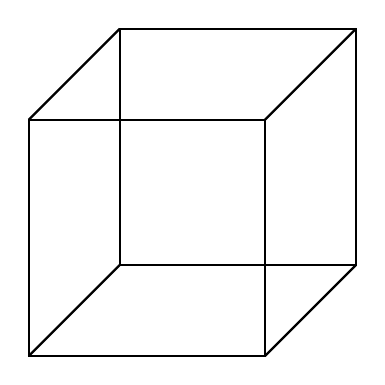
\begin{tikzpicture}[scale=3]
    % Coordonnées du cube
    \draw[thick] (0,0,0) -- (1,0,0) -- (1,1,0) -- (0,1,0) -- cycle; % Face inférieure
    \draw[thick] (0,0,1) -- (1,0,1) -- (1,1,1) -- (0,1,1) -- cycle; % Face supérieure
    \draw[thick] (0,0,0) -- (0,0,1); % Arête verticale
    \draw[thick] (1,0,0) -- (1,0,1); % Arête verticale
    \draw[thick] (1,1,0) -- (1,1,1); % Arête verticale
    \draw[thick] (0,1,0) -- (0,1,1); % Arête verticale
\end{tikzpicture}

\end{document}
